
%%--------------------------------------------------
%% CPO: Multiple Choice Questions
%%--------------------------------------------------


%% Chapter 5: Forces in Equilibrium
%%--------------------------------------------------


%% Learning Objectives
%%--------------------------------------------------

%% Draw vectors to scale to represent a quantity’s magnitude and direction. 
%% Solve vector problems. 
%% Find a vector’s components.
%% Explain what it means to say an object is in equilibrium. 
%% Use free-body diagrams to find unknown forces. 
%% Explain how springs exert forces.
%% Add force vectors. 
%% Distinguish between sliding and static friction.
%% Explain the cause of friction. 
%% Discuss reasons to increase or decrease friction. 
%% Explain how torque is created. 
%% Calculate torque on an object. 
%% Define rotational equilibrium.


%% CPO Multiple Choice Questions
%%--------------------------------------------------
\element{cpo-mc}{
\begin{question}{cpo-ch05-q01}
    A word meaning ``size'' often used to describe scalar quantities is:
    \begin{multicols}{2}
    \begin{choices}
        \wrongchoice{magma.}
        \wrongchoice{magenta.}
        \wrongchoice{vector.}
      \correctchoice{magnitude.}
    \end{choices}
    \end{multicols}
\end{question}
}

\element{cpo-mc}{
\begin{question}{cpo-ch05-q02}
    A measured quantity that is described by stating a size and a direction is called a:
    \begin{multicols}{2}
    \begin{choices}
        \wrongchoice{scalar}
        \wrongchoice{magnitude}
      \correctchoice{vector}
        \wrongchoice{victim}
    \end{choices}
    \end{multicols}
\end{question}
}

\element{cpo-mc}{
\begin{question}{cpo-ch05-q03}
    If a force vector acting in a northeast direction is resolved into its components,
        any vector acting in the north-south direction would be called a(n):
    \begin{multicols}{2}
    \begin{choices}
        \wrongchoice{hypotenuse}
        \wrongchoice{$x$-component}
      \correctchoice{$y$-component}
        \wrongchoice{resultant}
    \end{choices}
    \end{multicols}
\end{question}
}

\element{cpo-mc}{
\begin{question}{cpo-ch05-q04}
    Vector quantities include all of the following \emph{except}:
    \begin{multicols}{2}
    \begin{choices}
        \wrongchoice{velocity.}
        \wrongchoice{force.}
      \correctchoice{speed.}
        \wrongchoice{Acceleration.}
    \end{choices}
    \end{multicols}
\end{question}
}

\element{cpo-mc}{
\begin{question}{cpo-ch05-q05}
    A scalar is a quantity that can be completely described using:
    \begin{choices}
        \wrongchoice{direction only.}
      \correctchoice{magnitude only.}
        \wrongchoice{both magnitude and direction.}
        \wrongchoice{either magnitude and direction.}
    \end{choices}
\end{question}
}

\element{cpo-mc}{
\begin{question}{cpo-ch05-q06}   
    Jade pulls on a wagon with \SI{3}{\newton} of force toward north.
    Lara pulls on the wagon with \SI{4}{\newton} of force toward east.
    The magnitude of the wagon's resultant force is:
    \begin{multicols}{2}
    \begin{choices}
      \correctchoice{\SI{1}{\newton}.}
        \wrongchoice{\SI{5}{\newton}.}
        \wrongchoice{\SI{7}{\newton}.}
        \wrongchoice{\SI{25}{\newton}.}
    \end{choices}
    \end{multicols}
\end{question}
}

\element{cpo-mc}{
\begin{question}{cpo-ch05-q07}
    Forces in a diagram are represented by the following scale: \SI{1}{\centi\meter} equals \SI{5}{\newton}.
    To represent a force of \SI{20}{\newton},
        the length of an arrow drawn to represent the force should be:
    \begin{multicols}{2}
    \begin{choices}
        \wrongchoice{\SI{1}{\centi\meter}}
      \correctchoice{\SI{4}{\centi\meter}}
        \wrongchoice{\SI{5}{\centi\meter}}
        \wrongchoice{\SI{20}{\centi\meter}}
    \end{choices}
    \end{multicols}
\end{question}
}

\element{cpo-mc}{
\begin{question}{cpo-ch05-q08}
    Lily pushes a box with \SI{50}{\newton} toward east.
    Mia pushes on the same box with \SI{50}{\newton} toward south.
    The direction of the box's resultant force is most clearly stated as.
    \begin{multicols}{2}
    \begin{choices}
        \wrongchoice{\ang{45}}
        \wrongchoice{\ang{135}}
        \wrongchoice{\ang{225}}
      \correctchoice{\ang{315}}
    \end{choices}
    \end{multicols}
\end{question}
}

\element{cpo-mc}{
\begin{question}{cpo-ch05-q09}
    The diagram below represents a force acting at point $P$.
    \begin{center}
    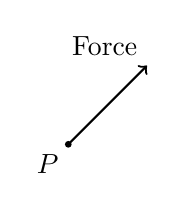
\begin{tikzpicture}
        \draw[fill=black] (0,0) circle (1pt);
        \draw[thick,->] (0,0) -- (45:1.414);
        \node[anchor=north east] at (0,0) {$P$};
        \node[anchor=south east] at (45:1.414) {Force};
    \end{tikzpicture}
    \end{center}
    The pair of forces that could represent $x$ and $y$ components of this force are:
    \begin{multicols}{2}
    \begin{choices}
        \AMCboxDimensions{down=-0.4cm}
        \wrongchoice{
            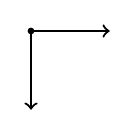
\begin{tikzpicture}
                \draw[fill=black] (0,0) circle (1pt);
                \draw[thick,->] (0,0) -- (0:1cm);
                \draw[thick,->] (0,0) -- (270:1cm);
            \end{tikzpicture}
        }
        \correctchoice{
            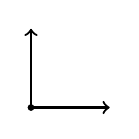
\begin{tikzpicture}
                \draw[fill=black] (0,0) circle (1pt);
                \draw[thick,->] (0,0) -- (90:1cm);
                \draw[thick,->] (0,0) -- (0:1cm);
            \end{tikzpicture}
        }
        \wrongchoice{
            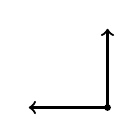
\begin{tikzpicture}
                \draw[fill=black] (0,0) circle (1pt);
                \draw[thick,->] (0,0) -- (90:1cm);
                \draw[thick,->] (0,0) -- (180:1cm);
            \end{tikzpicture}
        }
        \wrongchoice{
            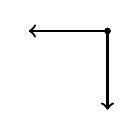
\begin{tikzpicture}
                \draw[fill=black] (0,0) circle (1pt);
                \draw[thick,->] (0,0) -- (180:1cm);
                \draw[thick,->] (0,0) -- (270:1cm);
            \end{tikzpicture}
        }
    \end{choices}
    \end{multicols}
\end{question}
}

\element{cpo-mc}{
\begin{question}{cpo-ch05-q10}
    Maya kicks a soccer ball \SI{2}{\newton} toward north.
    At the same time, Casey kicks the same ball toward west.
    The resultant force of the soccer ball is about \SI{36}{\newton}.
    The force that Casey kicks the soccer ball toward west is most nearly:
    \begin{multicols}{2}
    \begin{choices}
        \wrongchoice{\SI{16}{\newton}}
        \wrongchoice{\SI{20}{\newton}}
      \correctchoice{\SI{30}{\newton}}
        \wrongchoice{\SI{56}{\newton}}
    \end{choices}
    \end{multicols}
\end{question}
}

\element{cpo-mc}{
\begin{question}{cpo-ch05-q11}
    The relationship between a spring's change in length and the force it exerts is called:
    \begin{choices}
        \wrongchoice{Newton's law}
      \correctchoice{Hooke's law}
        \wrongchoice{Archimedes' principle}
        \wrongchoice{Galileo's theory}
    \end{choices}
\end{question}
}

\element{cpo-mc}{
\begin{question}{cpo-ch05-q12}   
    When a spring is compressed:
    \begin{choices}
      \correctchoice{the potential energy stored in the spring increases.}
        \wrongchoice{the potential energy stored in the spring decreases.}
        \wrongchoice{the spring constant of the spring is decreased.}
        \wrongchoice{the spring constant of the spring is increased.}
    \end{choices}
\end{question}
}

\element{cpo-mc}{
\begin{question}{cpo-ch05-q13}
    When the net force acting on an object is zero,
        this \emph{always} causes a condition of motion referred to as:
    \begin{choices}
        \wrongchoice{rest.}
        \wrongchoice{positive acceleration.}
        \wrongchoice{negative acceleration.}
      \correctchoice{equilibrium.}
    \end{choices}
\end{question}
}

\element{cpo-mc}{
\begin{question}{cpo-ch05-q14}
    when you are seated in a chair,
        the force exerted on you by the chair is called the:
    \begin{multicols}{2}
    \begin{choices}
      \correctchoice{normal force}
        \wrongchoice{gravitational force}
        \wrongchoice{weight}
        \wrongchoice{mass}
    \end{choices}
    \end{multicols}
\end{question}
}

\element{cpo-mc}{
\begin{question}{cpo-ch05-q15}
    A dictionary whose mass is \SI{1.0}{\kilo\gram} lying on a stationary table exerts a force of \SI{9.8}{\newton} on the table.
    The force on the dictionary by the table is:
    %% NOTE: this was incorrect in CPO document
    \begin{multicols}{2}
    \begin{choices}
        \wrongchoice{\SI{1.0}{\newton}}
        \wrongchoice{\SI{8.8}{\newton}}
      \correctchoice{\SI{9.8}{\newton}}
        \wrongchoice{\SI{10.8}{\newton}}
    \end{choices}
    \end{multicols}
\end{question}
}

%\element{cpo-mc}{
%\begin{question}{cpo-ch05-q16}
%    A car drives from east to west over a bridge supported by the ground
%        at either end as illustrated in the diagram:
%    \begin{center}
%    \end{tikzpicture}
%        %% NOTE: TODO: draw tikz??
%    \begin{tikzpicture}
%    \end{center}
%    The force exerted by the ground on the bridge at the west end is:
%    \begin{multicols}{2}
%    \begin{choices}
%        \wrongchoice{\SI{38}{tons}.}
%        \wrongchoice{\SI{39}{tons}.}
%      \correctchoice{\SI{20}{tons}.}
%        \wrongchoice{\SI{19}{tons}.}
%    \end{choices}
%    \end{multicols}
%\end{question}
%}

\element{cpo-mc}{
\begin{question}{cpo-ch05-q17}
    Eric is pedaling his bicycle due west on the Mohawk River bicycle path at a constant speed of \SI{17}{mile\per\hour}.
    As he is pedaling, a \SI{3}{mile\per\hour} wind is blowing from the east.
    The statement that best describes the forces acting on Eric's bicycle is:
    \begin{choices}
      \correctchoice{the net force acting on the bike is zero.}
        \wrongchoice{a greater net force is acting toward the east.}
        \wrongchoice{a greater net force is acting toward the west.}
        \wrongchoice{not enough information is given to answer the question.}
    \end{choices}
\end{question}
}

\element{cpo-mc}{
\begin{question}{cpo-ch05-q18}
    A force of \SI{2}{\newton} is required to stretch a spring \SI{4}{\centi\meter}.
    The amount of force required to stretch the same spring \SI{8}{\centi\meter} is:
    \begin{multicols}{2}
    \begin{choices}
        \wrongchoice{\SI{1}{\newton}}
        \wrongchoice{\SI{2}{\newton}}
      \correctchoice{\SI{4}{\newton}}
        \wrongchoice{\SI{8}{\newton}}
    \end{choices}
    \end{multicols}
\end{question}
}

\element{cpo-mc}{
\begin{question}{cpo-ch05-q19}
    If the stretching force on a spring is doubled,
        the length of the spring will be:
    \begin{multicols}{2}
    \begin{choices}
        \wrongchoice{unchanged}
      \correctchoice{doubled}
        \wrongchoice{quadrupled}
        \wrongchoice{halved}
    \end{choices}
    \end{multicols}
\end{question}
}

\element{cpo-mc}{
\begin{question}{cpo-ch05-q20}
    A spring with a large spring constant:
    \begin{choices}
        \wrongchoice{always stretches a large amount.}
        \wrongchoice{never stretches a large amount.}
        \wrongchoice{stretches a large distance with a small force.}
      \correctchoice{stretches a small distance with a large force.}
    \end{choices}
\end{question}
}

\element{cpo-mc}{
\begin{question}{cpo-ch05-q21}
    The force that resists the motion of objects or surfaces in contact with on another is called \rule[-0.1pt]{4em}{0.1pt} force.
    \begin{multicols}{2}
    \begin{choices}
        \wrongchoice{inertia}
      \correctchoice{frictional}
        \wrongchoice{normal}
        \wrongchoice{net}
    \end{choices}
    \end{multicols}
\end{question}
}

\element{cpo-mc}{
\begin{question}{cpo-ch05-q22}
    The force of friction between two surfaces can be reduced by all of the following \emph{except}:
    \begin{choices}
        \wrongchoice{separating surfaces with a lubricant.}
      \correctchoice{changing rolling friction to sliding friction.}
        \wrongchoice{separating surfaces with a layer of air.}
        \wrongchoice{sanding rough surfaces smoother.}
    \end{choices}
\end{question}
}

\element{cpo-mc}{
\begin{question}{cpo-ch05-q23}
    Two moving surfaces are in contact with one another.
    The force of friction between the surfaces can be changed by all of the following methods \emph{except}:
    \begin{choices}
        \wrongchoice{placing lubrication between the surfaces.}
        \wrongchoice{changing the types of surfaces.}
      \correctchoice{changing the force used to move the surfaces.}
        \wrongchoice{altering the force pushing the two surfaces together.}
    \end{choices}
\end{question}
}

\element{cpo-mc}{
\begin{question}{cpo-ch05-q24}
    To overcome static friction to start an object sliding on a level surface, a \SI{100}{\newton} force is used.
    The magnitude of the force needed to keep the object sliding is:
    \begin{choices}
        \wrongchoice{more than \SI{100}{\newton}.}
        \wrongchoice{equal to \SI{100}{\newton}.}
      \correctchoice{less than \SI{100}{\newton}.}
        \wrongchoice{unknown using the given information.}
    \end{choices}
\end{question}
}

\element{cpo-mc}{
\begin{question}{cpo-ch05-q25}
    Of the following, the statement about friction which is \emph{not} true is:
    \begin{choices}
        \wrongchoice{friction is always present}
        \wrongchoice{friction can be useful}
        \wrongchoice{friction can be harmful}
      \correctchoice{friction can be eliminated}
    \end{choices}
\end{question}
}

\element{cpo-mc}{
\begin{question}{cpo-ch05-q26}
    As Joshua accelerates in his pickup truck at \SI{2}{\meter\per\second\squared} a \SI{200}{\kilo\gram} box in the back does not slide.
    The force of friction that must act on the box to keep it from slipping in the back of the truck is:
    \begin{multicols}{2}
    \begin{choices}
        \wrongchoice{\SI{100}{\newton}}
        \wrongchoice{\SI{200}{\newton}}
      \correctchoice{\SI{400}{\newton}}
        \wrongchoice{\SI{1 960}{\newton}}
    \end{choices}
    \end{multicols}
\end{question}
}

%\element{cpo-mc}{
%\begin{question}{cpo-ch05-q27}
%    The diagram below represents a box sliding down an incline:
%    \begin{center}
%    \end{tikzpicture}
%        %% NOTE: TODO: draw tikz
%    \begin{tikzpicture}
%    \end{center}
%    The force of friction acting on the box is directed toward:
%    \begin{multicols}{2}
%    \begin{choices}
%        \wrongchoice{\num{1}.}
%      \correctchoice{\num{2}.}
%        \wrongchoice{\num{3}.}
%        \wrongchoice{\num{4}.}
%    \end{choices}
%    \end{multicols}
%\end{question}
%}

\element{cpo-mc}{
\begin{question}{cpo-ch05-q28}
    Pulling on a rope with a force of \SI{100}{\newton} at an angle \ang{30},
        Cheung pulls a box across a surface at a constant speed.
    \begin{center}
    \begin{tikzpicture}
        \draw[very thick] (-2,0) -- (2,0);
        \draw[very thick] (-1,0) rectangle (0,1);
        \draw[very thick,->] (0,0.5) -- ++(30:2)
            node[pos=0.66,rotate=30,anchor=south] {\SI{100}{\newton}};
        \draw[dashed] (0,0.5) -- (1.73,0.5);
        \draw[->,dashed] (1,0.5) arc (0:30:1)
            node[pos=0.5,anchor=west] {\ang{30}};
    \end{tikzpicture}
    \end{center}
    The magnitude of the frictional force resisting the motion is:
    \begin{multicols}{2}
    \begin{choices}
        \wrongchoice{\SI{100}{\newton}}
      \correctchoice{\SI{87}{\newton}}
        \wrongchoice{\SI{50}{\newton}}
        \wrongchoice{\SI{0}{\newton}}
    \end{choices}
    \end{multicols}
\end{question}
}

\element{cpo-mc}{
\begin{question}{cpo-ch05-q29}
    The line about which an object turns is called the:
    \begin{multicols}{2}
    \begin{choices}
        \wrongchoice{torque.}
      \correctchoice{axis of rotation.}
        \wrongchoice{radius.}
        \wrongchoice{lever arm.}
    \end{choices}
    \end{multicols}
\end{question}
}

\element{cpo-mc}{
\begin{question}{cpo-ch05-q30}
    As the force applied to a rotating object is moved farther from the axis of rotation,
        the torque created by the force:
    \begin{choices}
      \correctchoice{increases.}
        \wrongchoice{decreases.}
        \wrongchoice{is always clockwise.}
        \wrongchoice{is always perpendicular to the lever arm.}
    \end{choices}
\end{question}
}

\element{cpo-mc}{
\begin{question}{cpo-ch05-q31}
    Aaron applies a \SI{70.0}{\newton} force to the handle of a wrench at a distance of \SI{0.350}{\meter} from the nut on the axle of his bicycle wheel.
    The amount of torque applied to the nut is:
    \begin{multicols}{2}
    \begin{choices}
        \wrongchoice{\SI{0.005}{\newton\meter}}
      \correctchoice{\SI{24.5}{\newton\meter}}
        \wrongchoice{\SI{70.35}{\newton\meter}}
        \wrongchoice{\SI{200}{\newton\meter}}
    \end{choices}
    \end{multicols}
\end{question}
}

%\element{cpo-mc}{
%\begin{question}{cpo-ch05-q32}
%    The diagram reprsents a lever to which forces are applied:
%    \begin{center}
%    \end{tikzpicture}
%        %% NOTE: TODO: draw tikz
%    \begin{tikzpicture}
%    \end{center}
%    To create rotational equilibrium, the force exerted at the left
%        end of the lever must be:
%    \begin{multicols}{2}
%    \begin{choices}
%        \wrongchoice{\SI{36}{\newton}.}
%        \wrongchoice{\SI{27}{\newton}.}
%      \correctchoice{\SI{12}{\newton}.}
%        \wrongchoice{\SI{4}{\newton}.}
%    \end{choices}
%    \end{multicols}
%\end{question}
%}

%\element{cpo-mc}{
%\begin{question}{cpo-ch05-q33}
%    Juan and his younger sister Ana are able to balance when seated on a see-saw.
%    Juan weights \SI{800}{newton} and sits \SI{2.0}{\meter} from the balance point.
%    Ana weighs \SI{400}{\newton}.
%    \begin{center}
%    \end{tikzpicture}
%        %% NOTE: TODO: draw tikz
%    \begin{tikzpicture}
%    \end{center}
%    To create rotational equilibrium, the distance she must sit from the
%        balance point is:
%    \begin{multicols}{2}
%    \begin{choices}
%        \wrongchoice{\SI{1.0}{\meter}.}
%        \wrongchoice{\SI{2.0}{\meter}.}
%      \correctchoice{\SI{4.0}{\meter}.}
%        \wrongchoice{\SI{8.0}{\meter}.}
%    \end{choices}
%    \end{multicols}
%\end{question}
%}


\endinput


